%!TEX root = brainreader.tex

\section{Methods}

Our processing pipeline takes as input two pieces of data for each second:

\begin{itemize}
\item The top 100 guesses (based on fMRI data) - each guess has 15 frames
\item The log-likelihood (LLH) of each guess
\end{itemize}

We experimented with a variety of options for the 5 core steps of \emph{Weeding}, \emph{Forced Alignment}, \emph{Flow Calculation}, \emph{Pathfinding}, and \emph{Visualization} (see Figure \ref{fig:system}).

\begin{figure}
\centering
    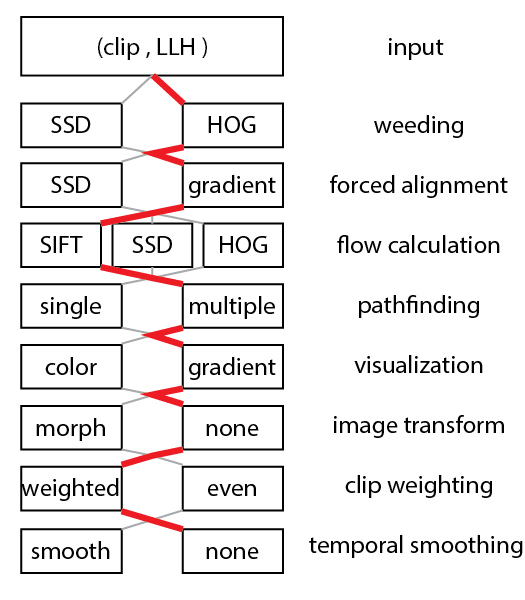
\includegraphics[width=1.0\columnwidth]{figures/system.png}
\caption{We experimented with a variety of options for the core steps of Preprocessing, Forced Alignment, Flow Calculation, Pathfinding, and Visualization (including method, image transformation, clip weighting, and temporal smoothing).  Highlighted in red is the path that was chosen.}
\label{fig:system}
\end{figure}

There are a few processes that we used for several steps in our pipeline, described here for later reference:

\emph{SSD} - Sum of Squared Differences (SSD) is a single number that represents a ``match'' score between two images.  It takes into account differences across the images' respective color channels, squaring and summing those differences to create one number indicating overall different-ness.

\emph{HOG} - Histogram of Oriented Gradients (HOG) descriptors focus on an image's edge data.  The descriptor has a variety of bins representing orientations and locations: images with similar HOG descriptors have similar edge orientations in similar spatial locations \cite{HOG}.

\emph{Gradient} - An image's gradient magnitude is equal to the square root of the sum of squares of the x-gradient and y-graident and represents change in the image rather than absolute values.  Large changes in the image typically correspond to edges.

\subsection{Weeding}
While the 100 clips are already chosen to correspond to the fMRI data by the log-likelihood values of the model, in order to make an effective visualization we first discard clips that have very jarring transitions between timepoints. By minimizing the change in the content of the first frame of each clip and the last frame of the previous clip, we smooth the set of clips to one with smoother transitions.

We attempted two processes for this: \emph{SSD} and \emph{HOG}.  Intuitively, SSD should be better for preserving color across clips, since it takes color into account, while HOG should be better at preserving the edge content from one clip to another.  Therefore, we would expect that HOG-weeded guess clips would have better shape consistency.  This appears to be true to some degree (see Figure \ref{fig:weeding}): therefore we select HOG as our weeding tool of choice (in spite of SSD's obvious superiority in time efficiency).

\begin{figure}
\centering
    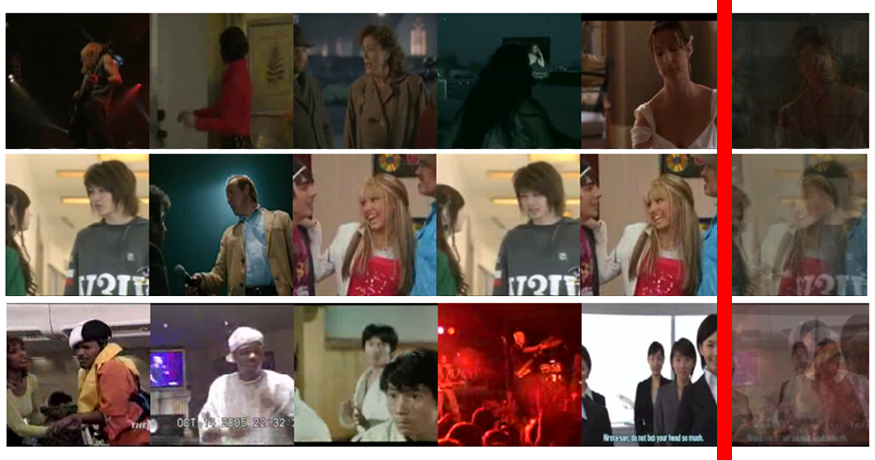
\includegraphics[width=1.0\columnwidth]{figures/preproc.png}
\caption{The top 5 guesses for one frame weeded based on SSD (top), HOG (middle), and LLH (bottom); and the sum of all five images (right).}
\label{fig:weeding}
\end{figure}

\subsection{Forced Alignment}
We forcibly align our guesses to each other: this makes the final visualization more pleasing, in addition to making flow calculations (discussed next) more meaningful. This precision of decoded alignment cannot be exact with fMRI data, and thus this alignment is justified. Although some neurons, particularly in early visual areas, are tuned precisely to very small portions of the visual field, fMRI voxels average over hundreds of thousands of neurons, and such fine tuning is lost. Nonetheless, voxels are spatially tuned, well enough to recover retinotopic organization of the visual areas, but this tuning is at less than pixel accuracy. Thus we can improve our visualization by alignment at a pixel level.

The two forced alignment metrics we tested were \emph{SSD} and \emph{gradient}.

SSD-based alignment forcing encourages alignment of colors, while gradient-based alignment encourages alignment of edges.  Depending on the final visualization configuration, either may be desirable: if the visualization is going to be compiled in the color domain, color-based alignment may be best.  However, alignment in the gradient domain is more suited to visualization in the gradient domain (see Figure \ref{fig:align}).

\begin{figure}
\centering
    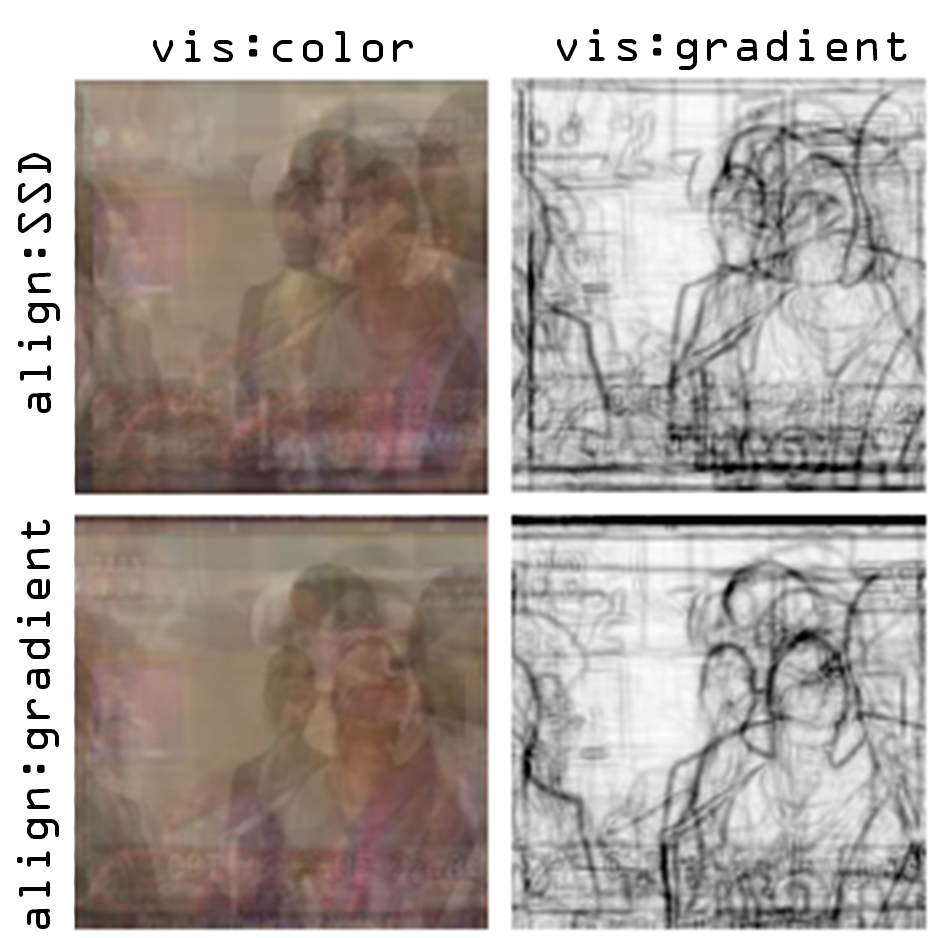
\includegraphics[width=1.0\columnwidth]{figures/align.png}
\caption{SSD-based alignment and gradient-based alignment lend themselves to different visualization techniques.  Here we show all possibilities of alignment technique x visualization technique: note that the lines match up best in the gradient domain when alignment is done there, and colors match up best when SSD is the alignment technique.}
\label{fig:align}
\end{figure}

For our final videos, we selected to use gradient-based alignment: visualizing our output in the gradient domain is more ``true'' to the fMRI data, which only accounts for shape and ignores color, and gradient-based alignment lends itself to gradient-based visualization.

\subsection{Flow Calculation}
We elected to reduce the number of clips shown in the final visualization from 100 to a much smaller number, which allows us some additional flexibility in stringing the clips together.  Instead of needing to create transitions from every clip from one time step into every clip from the next time step, we are able to take one or a few clips from the 100 best guesses and create a smooth path through those clips.

But what makes a ``smooth'' path?  Ideally, a smooth path is one where the last frame of one clip lines up with the first frame of the following clip: various techniques have been tried to determine the ``difference'' between two images.

\emph{SIFT flow} \cite{SIFTflow} finds SIFT keypoints in two images and estimates the ``flow'' of these keypoints between the two images. This type of matching rewards scenes that are semantically, though perhaps not compositionally, similar: e.g., two images of streets would likely have low SIFT flow, while an image with a street at the bottom and an image with a river at the bottom would likely have high SIFT flow.  We found the smoothest paths using SIFT flow. Unfortunately, it is much more computationally expensive than other techniques we tried, but the improvement was much greater.

A second technique for path smoothness is \emph{SSD}.  Used in this part of the pipeline, SSD will ideally minimize jumps in color and composition between adjacent time steps, making clips flow smoothly into each other.

The final flow calculation we implemented was \emph{HOG}-based flow.  This again focuses on edge orientation and location, and lends itself to visualization consistency in the gradient domain.

Both the SSD and HOG techniques are the same as the ones we tried above before aligning the images. Thus, we only use the weeding step for the SIFT flow version of this step.

We compare the various flow calculation techniques tested in Figure \ref{fig:flows}.

\begin{figure}
\centering
    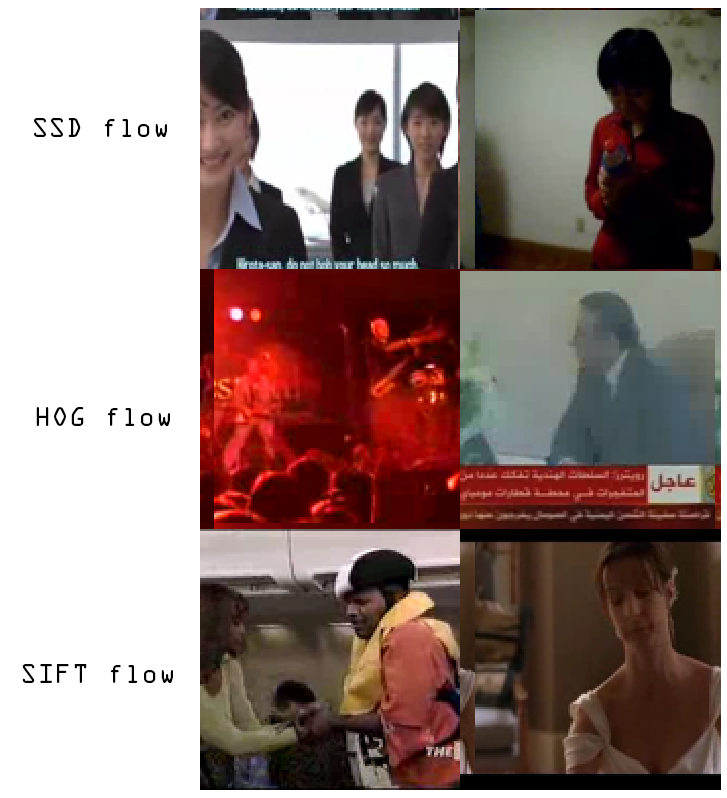
\includegraphics[width=1.0\columnwidth]{figures/lowflowstitled.png}
\caption{Various techniques can be used to calculate the ``difference'' between two images (in our case, the last frame of one clip and the first frame of the following clip).  We implemented SSD (focus on colors), HOG (focus on edges), and SIFT (focus on semantics).}
\label{fig:flows}
\end{figure}


\subsection{Pathfinding}
To find the optimal path through the clips, the whole set of clips can be seen as a Markov chain. There is a node at each second of the reconstructed movie, and the possible clips for that second representing the states of that node. The flow metrics between each pair of clips constitue the values of the transition matrix between all states. We used dynamic programming to find the optimal path through the transition matrix. First, we found the lowest cumulative cost to get to each consecutive clip in the transition matrix. Then, we backtracked through the transition cost matrix to find the cheapest path for one or several clips. After some testing, we chose a path of five clips, as it produced the most visually appealing results.

\subsection{Visualization}
We visualized the resuling movies in several ways. First, we averaged the clips in the chosen path to obtain one continuous movie. This gave us the most direct comparison to the previous approach of averaging the top 100 clips. Before averaging, we weighted the clips by the relative fMRI model log-likelihood of each clip. See Figure \ref{fig:viz} (a).

\subsubsection{Gradient Domain and Overlay}
The fMRI model is based on spatiotemporal features of the movies, including spatial frequencies and orientations. We wanted to emphasize the decoding of these features by highlighting the edges in the reconstructed movies. To do this, we visualized the reconstructed movies in the gradient domain. The gradient magnitude of all clips was computed. We displayed the inverse magnitude, showing dark edges on a white background. To demonstrate the difference between the reconstructed and original movie, we also computed the gradient of the original movie. We overlayed the original gradient movie in red over the reconstructed gradient movie in black and white. See Figure \ref{fig:viz} (b) and (c).

\begin{figure}
\centering
    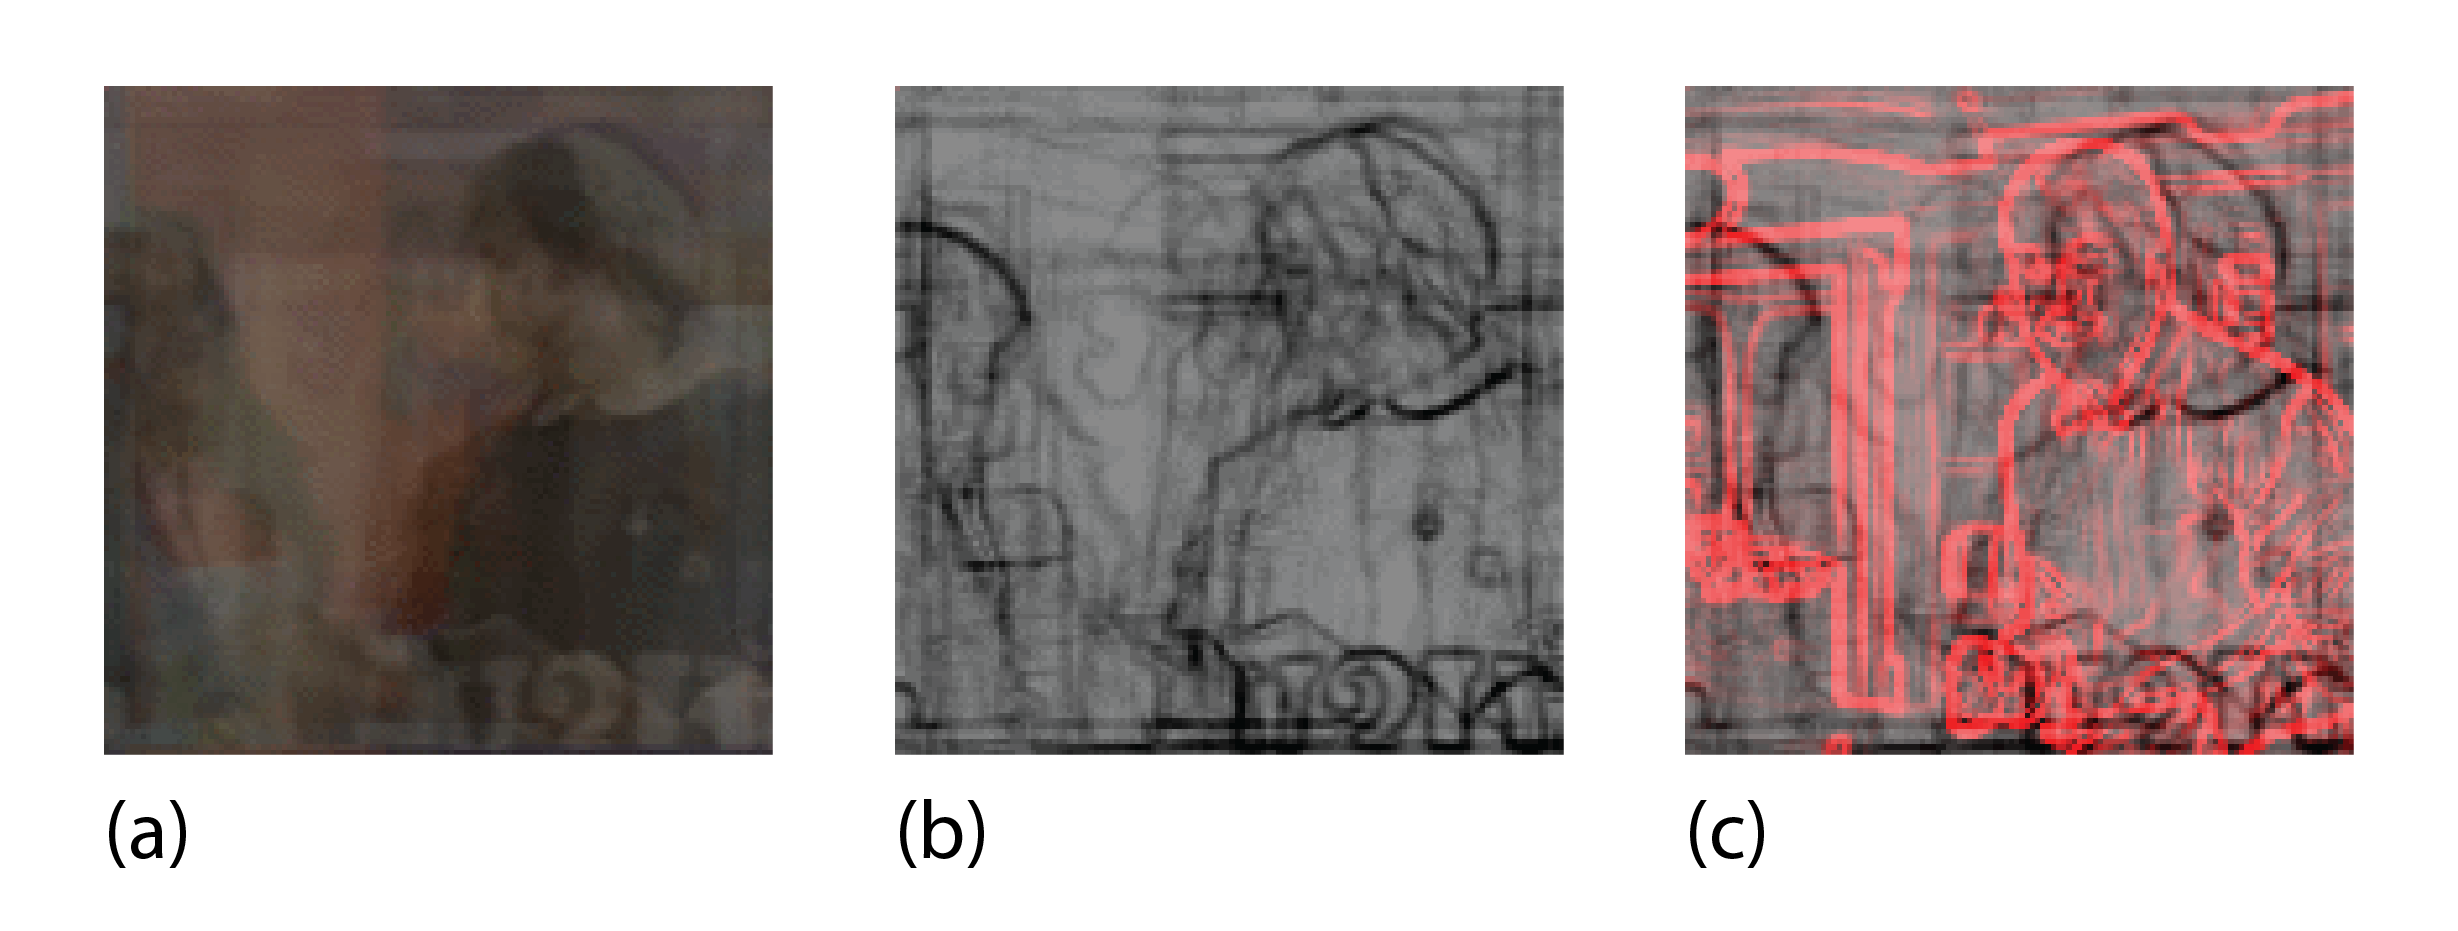
\includegraphics[width=1.0\columnwidth]{figures/vizfig.png}
\caption{Three techniques were used to visualize the results. (a) Top 5 clips found in the smoothest path, weighted by relative log-likelihood and averaged. (b) The same 5 clips, transformed to gradient magnitude before averaging. (c) The same result, withg the radient magnitude of the original clip overlaid in red.}
\label{fig:viz}
\end{figure}

\subsubsection{Smoothing}
To make the appearance of the movie smoother, we averaged the clips temporally with a moving average filter. The averaging was done with each frame weighted by the reciprocal of the window width. We experimented with several sliding window width and chose five frames as the best span.